\documentclass[tikz,border=2pt]{standalone}
\usepackage{amsmath}
\usepackage{amssymb}
\usepackage{pgfplots}
\pgfplotsset{compat=1.18}
\usetikzlibrary{arrows.meta}
\begin{document}
% Algorithm 6.2 as a flow diagram: step 1 (feasible basis, B^{-1}) -> step 2 (reduced costs from c_B^T B^{-1})
% -> step 3 (pivot column B^{-1}A_{j*}) -> step 4 (minimum-ratio test) -> step 5 (exchange, update B^{-1})
% -> step 6 (x_B = B^{-1}b, Z) -> step 7 back to step 2; exits: infeasible (1), optimal (2), unbounded (3).
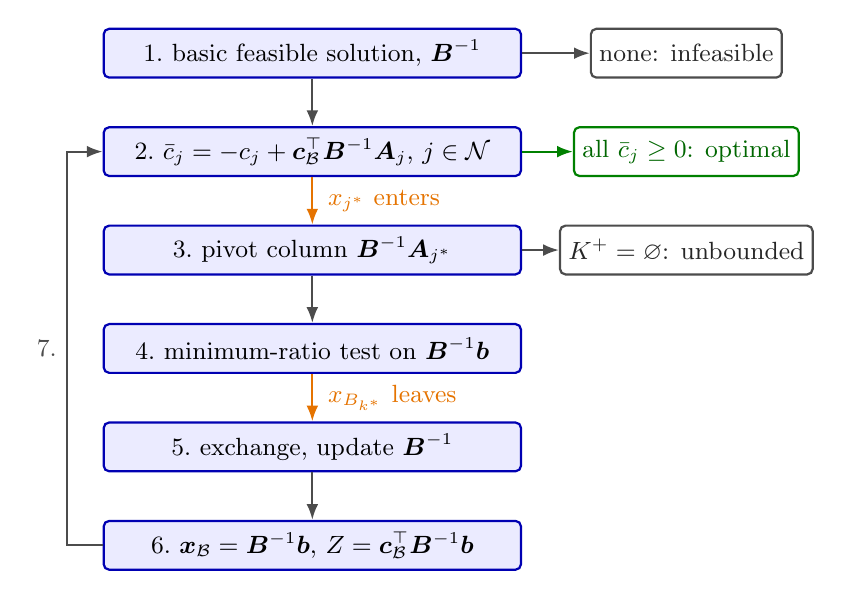
\begin{tikzpicture}[font=\small, >={Latex[length=2mm]},
    algstep/.style={draw=blue!70!black, thick, rounded corners=2pt, fill=blue!8, minimum width=5.3cm, minimum height=0.62cm, inner sep=3pt},
    stop/.style={draw, thick, rounded corners=2pt, minimum height=0.62cm, inner sep=3pt, align=center}]
  \node[algstep] (s1) at (0,0) {1.\ basic feasible solution, $\boldsymbol{B}^{-1}$};
  \node[algstep] (s2) at (0,-1.25) {2.\ $\bar{c}_j=-c_j+\boldsymbol{c}_{\mathcal{B}}^{\top}\boldsymbol{B}^{-1}\boldsymbol{A}_j$, $j\in\mathcal{N}$};
  \node[algstep] (s3) at (0,-2.5) {3.\ pivot column $\boldsymbol{B}^{-1}\boldsymbol{A}_{j^*}$};
  \node[algstep] (s4) at (0,-3.75) {4.\ minimum-ratio test on $\boldsymbol{B}^{-1}\boldsymbol{b}$};
  \node[algstep] (s5) at (0,-5.0) {5.\ exchange, update $\boldsymbol{B}^{-1}$};
  \node[algstep] (s6) at (0,-6.25) {6.\ $\boldsymbol{x}_{\mathcal{B}}=\boldsymbol{B}^{-1}\boldsymbol{b}$, $Z=\boldsymbol{c}_{\mathcal{B}}^{\top}\boldsymbol{B}^{-1}\boldsymbol{b}$};
  % main flow
  \draw[->, thick, gray!60!black] (s1) -- (s2);
  \draw[->, thick, orange!90!black] (s2) -- node[anchor=west, xshift=2pt] {$x_{j^*}$ enters} (s3);
  \draw[->, thick, gray!60!black] (s3) -- (s4);
  \draw[->, thick, orange!90!black] (s4) -- node[anchor=west, xshift=2pt] {$x_{B_{k^*}}$ leaves} (s5);
  \draw[->, thick, gray!60!black] (s5) -- (s6);
  % step 7: back to step 2
  \draw[->, thick, gray!60!black] (s6.west) -- ++(-0.45,0) |- node[pos=0.25, anchor=east] {7.} (s2.west);
  % exits
  \node[stop, draw=gray!60!black, text=gray!30!black] (e1) at (4.75,0) {none: infeasible};
  \node[stop, draw=green!50!black, text=green!40!black] (e2) at (4.75,-1.25) {all $\bar{c}_j\geq0$: optimal};
  \node[stop, draw=gray!60!black, text=gray!30!black] (e3) at (4.75,-2.5) {$K^{+}=\varnothing$: unbounded};
  \draw[->, thick, gray!60!black] (s1) -- (e1);
  \draw[->, thick, green!50!black] (s2) -- (e2);
  \draw[->, thick, gray!60!black] (s3) -- (e3);
\end{tikzpicture}
\end{document}
